%% Los cap'itulos inician con \chapter{T'itulo}, estos aparecen numerados y
%% se incluyen en el 'indice general.
%%
%% Recuerda que aqu'i ya puedes escribir acentos como: 'a, 'e, 'i, etc.
%% La letra n con tilde es: 'n.
\chapter{Resultados}
\section{Paquete de R \emph{geneticae}}

El paquete \emph{geneticae} permite analizar datos provenientes de etapas avanzadas de los programas de mejoramiento, donde se evalúan pocos genotipos. 

Una vez instalado el paquete, se debe cargar en la sesion de R mediante el comando: \textcolor{blue}{library}(geneticae)

Es posible obtener información detallada sobre las funciones del paquete geneticae mediante \textcolor{blue}{help}(package = "geneticae").  La ayuda para una función, por ejemplo, \textcolor{blue}{imputation}(), en una sesión R se puede obtener usando \emph{?imputation} o \textcolor{blue}{help}(imputation). Además, a partir de la función \textcolor{blue}{browseVignettes}("geneticae") se obtiene la viñeta del paquete, es decir una descripción el problema que está diseñado para resolver asi como ejemplos de aplicación del mismo.


\subsection{Conjuntos de datos en geneticae}

El paquete geneticae proporciona dos conjuntos de datos para ilustrar la metodología incluida para analizar los datos obtenidos de EMA.

\begin{itemize}[wide, nosep, labelindent = 0pt, topsep = 1ex]
\item yan.winterwheat dataset: rendimiento de 18 variedades de trigo de invierno cultivadas en nueve ambientes en Ontario en 1993. No hay réplicas disponibles en los datos. Este conjunto de datos se obtuvo del paquete agridat.

\begin{tcolorbox}[skin=bicolor,
    colframe=aurometalsaurus,colback=backcolour,colbacklower=white,
    width=1\linewidth,
    height=0.4\linewidth,
    boxsep=-3mm]
\begin{lstlisting}[linewidth=\columnwidth]
data(yan.winterwheat)
dat_yan <- yan.winterwheat
head(dat_yan)
\end{lstlisting}

\tcblower\vskip-\baselineskip
\tcblower
\vspace{0.5cm}
\footnotesize\begin{verbatim}
##   gen  env yield
## 1 Ann BH93 4.460
## 2 Ari BH93 4.417
## 3 Aug BH93 4.669
## 4 Cas BH93 4.732
## 5 Del BH93 4.390
## 6 Dia BH93 5.178
\end{verbatim}
\end{tcolorbox}

\item plrv dataset: rendimiento, peso de planta y parcela de 28 clones de la población del virus del enrollamiento de la papa (PLRV) evaluada en seis ambientes. Las réplicas están disponibles en los datos. Este conjunto de datos se obtuvo del paquete agricolae.

\begin{tcolorbox}[skin=bicolor,
    colframe=aurometalsaurus,colback=backcolour,colbacklower=white,
    width=1\linewidth,
    height=0.4\linewidth,
    boxsep=-3mm]
\begin{lstlisting}
data(plrv)
dat_rep <- plrv
head(dat_rep)
\end{lstlisting}

\tcblower\vskip-\baselineskip
\tcblower
\vspace{0.5cm}
\footnotesize\begin{verbatim}
##   Genotype Locality Rep WeightPlant WeightPlot    Yield
## 1   102.18     Ayac   1   0.5100000       5.10 18.88889
## 2   104.22     Ayac   1   0.3450000       2.76 12.77778
## 3   121.31     Ayac   1   0.5425000       4.34 20.09259
## 4   141.28     Ayac   1   0.9888889       8.90 36.62551
## 5   157.26     Ayac   1   0.6250000       5.00 23.14815
## 6    163.9     Ayac   1   0.5120000       2.56 18.96296
\end{verbatim}
\end{tcolorbox} 
 
\end{itemize}
 
 
 
\subsection{Funciones en geneticae}

\textbf{Modelo de regresión por sitio}

Para ejecutar la función \textcolor{blue}{GGEmodel}(), se debe proporcionar un conjunto de datos con genotipos, ambientes, repeticiones (si hay disponibles), el fenotipo observado y los nombres que dichas variables tienen en el archivo de entrada. Además, se debe indicar el método de centrado, escala y SVD.

Cuando no hay repeticiones disponibles en el conjunto de datos, como es el caso del conjunto de datos yan.winterwheat, el modelo GGE se indica de la siguiente manera:
\begin{tcolorbox}[colframe=aurometalsaurus,colback=backcolour,colbacklower=white,
    width=1\linewidth,
    height=0.1\linewidth,
    boxsep=-3mm]
\begin{lstlisting}
GGE1 <- GGEmodel(dat_yan, genotype = "gen", environment = "env", response = "yield", centering = "tester")
\end{lstlisting}
\end{tcolorbox}
Sin embargo, en el caso de que haya repeticiones disponibles, como el conjunto de datos plrv, se indica de la siguiente manera:

\begin{tcolorbox}[colframe=aurometalsaurus,colback=backcolour,colbacklower=white,
    width=1\linewidth,
    height=0.1\linewidth,
    boxsep=-3mm]
\begin{lstlisting}
GGE1_rep <- GGEmodel(dat_rep, genotype = "Genotype", environment = "Locality", response = "Yield", rep = "Rep", centering = "tester")
\end{lstlisting}
\end{tcolorbox}

La salida de la función \textcolor{blue}{GGEmodel}() es una lista con los siguientes elementos:

\begin{itemize}[wide, nosep, labelindent = 0pt, topsep = 1ex]
\item coordgenotype: trazado de coordenadas para genotipos de todos los componentes.
\item coordenviroment: trazado de coordenadas para entornos de todos los componentes.
\item valores propios: vector de valores propios de cada componente.
\item vartotal: varianza general.
\item varexpl: porcentaje de varianza explicado por cada componente.
\item labelgen: nombres de genotipo.
\item labelenv: nombres de entorno.
\item ejes: etiquetas de eje.
\item Datos: datos de entrada escalados y centrados.
\item centrado: nombre del método de centrado.
\item escala: nombre del método de escala.
\item SVP: nombre del método SVP.
\end{itemize}

\textbf{Biplot GGE}

Para ejecutar la función \textcolor{blue}{GGEPlot}(), se requiere un objeto de la clase \textcolor{blue}{GGEmodel}(). La salida es un biplot construido a través de los componentes principales generados por \textcolor{blue}{GGEmodel}().
Los diferentes biplots que se pueden obtener usando la función \textcolor{blue}{GGEPlot}() se muestran usando el conjunto de datos yan.winterwheat. Si hay repeticiones disponibles en el conjunto de datos, como es el caso del conjunto plrv, se debe indicar el nombre de la columna que contiene las réplicas en el archivo de entrada.

\begin{itemize}[wide, nosep, labelindent = 0pt, topsep = 1ex]
\item Biplot básico
\begin{tcolorbox}[skin=bicolor,
    colframe=aurometalsaurus,colback=backcolour,colbacklower=white,
    width=1\linewidth,
    height=0.7\linewidth,
    boxsep=-3mm]
\begin{lstlisting}
GGEPlot(GGE1, type = "Biplot")
\end{lstlisting}

\tcblower\vskip-\baselineskip
\tcblower
\begin{figure}[H]
	\begin{center}
		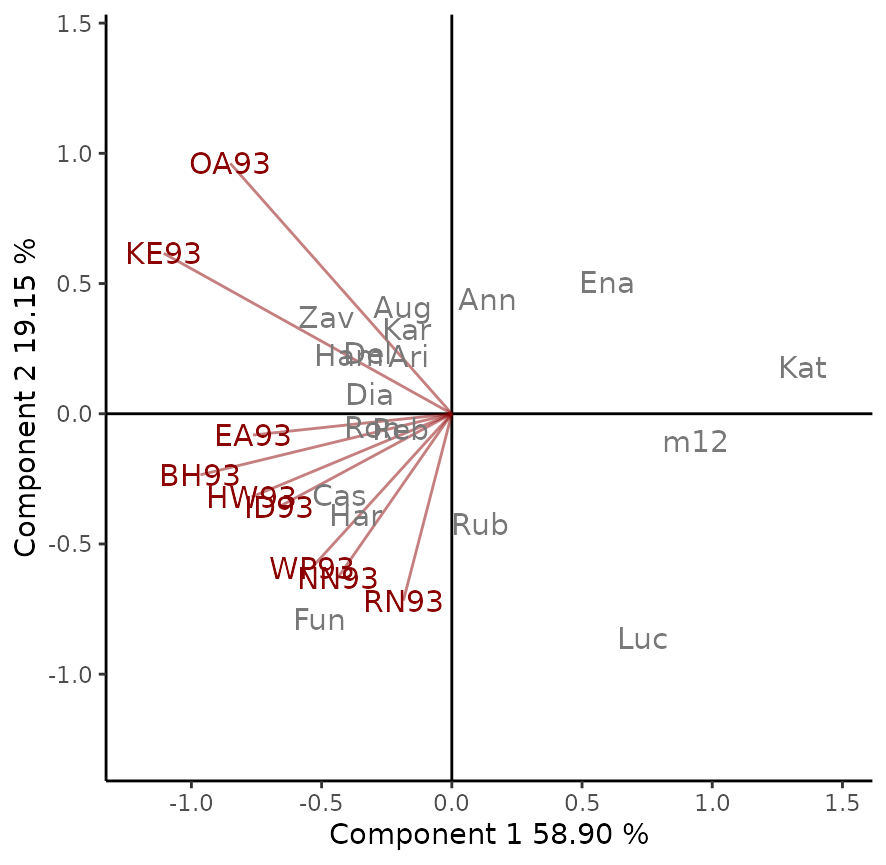
\includegraphics[width=8cm]{./Graficos/GGE_BIPLOT.png}
	\end{center}
	\caption{Biplot básico obtenido de la función \textcolor{blue}{GGEPlot}()}
\end{figure}
\end{tcolorbox} 

\item Ranking de los cultivares en función de su rendimiento en el ambiente OA93.
\begin{tcolorbox}[skin=bicolor,
    colframe=aurometalsaurus,colback=backcolour,colbacklower=white,
    width=1\linewidth,
    height=0.7\linewidth,
    boxsep=-3mm]
\begin{lstlisting}
GGEPlot(GGE1, type = "Selected Environment", selectedE = "OA93")
\end{lstlisting}

\tcblower\vskip-\baselineskip
\tcblower

\begin{figure}[H]
	\begin{center}
		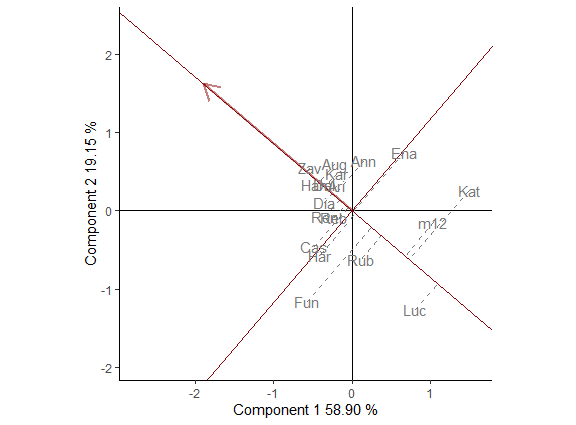
\includegraphics[width=8cm]{./Graficos/SelectedEnvironment.png}
	\end{center}
	\caption{Ranking de cultivares para un ambiente determinado obtenido de la función \textcolor{blue}{GGEPlot}()}
\end{figure}
\end{tcolorbox} 

\item Ranking de los ambientes en función del rendimiento relativo del cultivar Kat.
\begin{tcolorbox}[skin=bicolor,
    colframe=aurometalsaurus,colback=backcolour,colbacklower=white,
    width=1\linewidth,
    height=0.7\linewidth,
    boxsep=-3mm]
\begin{lstlisting}
GGEPlot(GGE1, type = "Selected Genotype", selectedG = "Kat")
\end{lstlisting}
\tcblower\vskip-\baselineskip
\tcblower
\begin{figure}[H]
	\begin{center}
		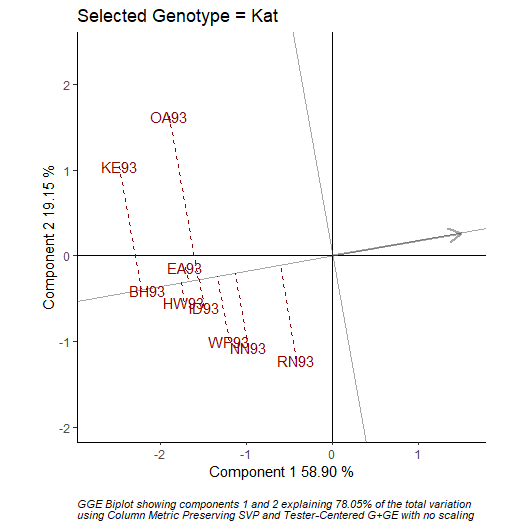
\includegraphics[width=8cm]{./Graficos/SelectedGenotype.png}
	\end{center}
	\caption{Ranking de ambientes para cultivar determinado obtenido de la función \textcolor{blue}{GGEPlot}()}
\end{figure}
\end{tcolorbox} 
\item Relación entre ambientes.
\begin{tcolorbox}[skin=bicolor,
    colframe=aurometalsaurus,colback=backcolour,colbacklower=white,
    width=1\linewidth,
    height=0.7\linewidth,
    boxsep=-3mm]
\begin{lstlisting}
GGEPlot(GGE1, type = "Relationship Among Environments")
\end{lstlisting}
\tcblower\vskip-\baselineskip
\tcblower
\begin{figure}[H]
	\begin{center}
		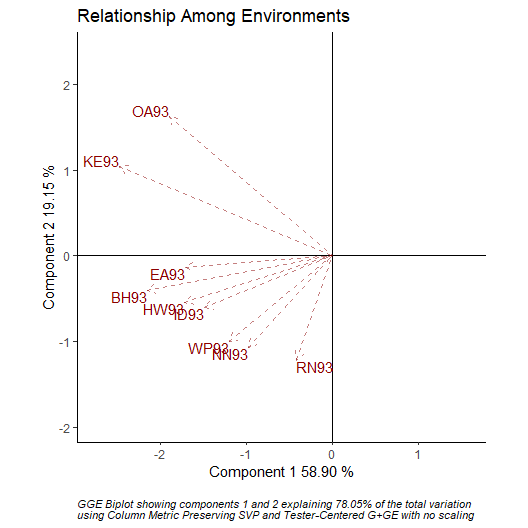
\includegraphics[width=8cm]{./Graficos/RelationshipAmongEnvironments.png}
	\end{center}
	\caption{Relación entre ambientes obtenido de la función \textcolor{blue}{GGEPlot}()}
\end{figure}
\end{tcolorbox}
\item Comparación entre los genotipos Kat y Cas.
\begin{tcolorbox}[skin=bicolor,
    colframe=aurometalsaurus,colback=backcolour,colbacklower=white,
    width=1\linewidth,
    height=0.7\linewidth,
    boxsep=-3mm]
\begin{lstlisting}
GGEPlot(GGE1, type = "Comparison of Genotype", selectedG1 = "Kat", selectedG2 = "Cas")
\end{lstlisting}
\tcblower\vskip-\baselineskip
\tcblower
\begin{figure}[H]
	\begin{center}
		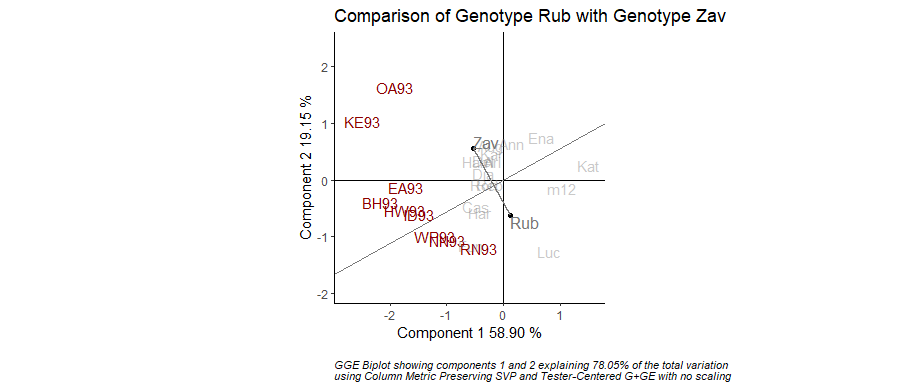
\includegraphics[width=8cm]{./Graficos/ComparisonofGenotype.png}
	\end{center}
	\caption{Comparación entre dos genotipos obtenido de la función \textcolor{blue}{GGEPlot}()}
\end{figure}
\end{tcolorbox}
\item Identificación del mejor cultivar en cada ambiente.
\begin{tcolorbox}[skin=bicolor,
    colframe=aurometalsaurus,colback=backcolour,colbacklower=white,
    width=1\linewidth,
    height=0.7\linewidth,
    boxsep=-3mm]
\begin{lstlisting}
GGEPlot(GGE1, type = "Which Won Where/What")
\end{lstlisting}
\tcblower\vskip-\baselineskip
\tcblower
\begin{figure}[H]
	\begin{center}
		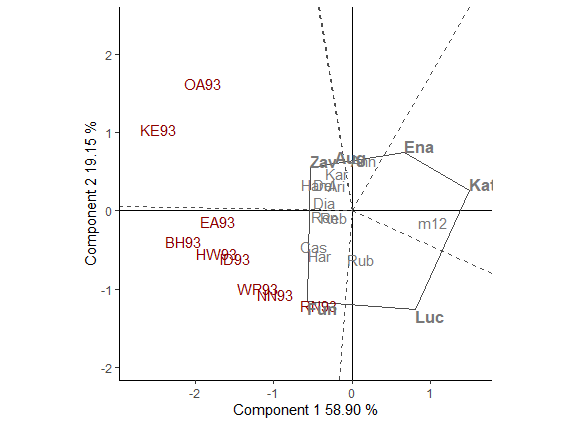
\includegraphics[width=8cm]{./Graficos/WhichWonWhereWhat.png}
	\end{center}
	\caption{Identificación del mejor cultivar en cada ambiente a partir de la función \textcolor{blue}{GGEPlot}()}
\end{figure}
\end{tcolorbox}
\item Evaluación de los ambientes basados tanto en la capacidad de discriminación como en la representatividad.
\begin{tcolorbox}[skin=bicolor,
    colframe=aurometalsaurus,colback=backcolour,colbacklower=white,
    width=1\linewidth,
    height=0.7\linewidth,
    boxsep=-3mm]
\begin{lstlisting}
GGEPlot(GGE1, type = "Discrimination vs. representativeness")
\end{lstlisting}
\tcblower\vskip-\baselineskip
\tcblower
\begin{figure}[H]
	\begin{center}
		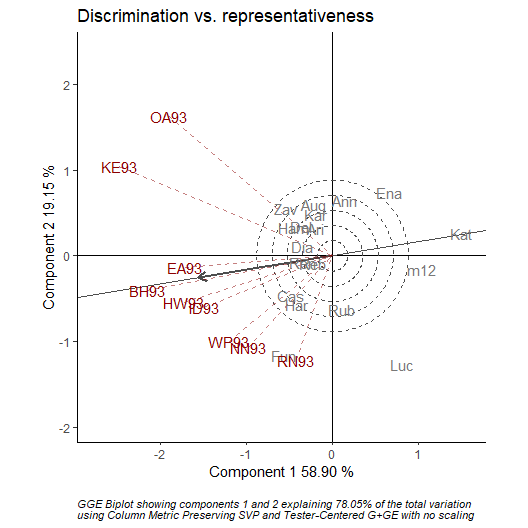
\includegraphics[width=8cm]{./Graficos/Discriminationvsrepresentativeness.png}
	\end{center}
	\caption{Evaluación de los ambientes basados tanto en la capacidad de discriminación y representatividad a partir de la función \textcolor{blue}{GGEPlot}()}
\end{figure}
\end{tcolorbox}
\item Clasificación de ambientes con respecto al ambiente ideal.
\begin{tcolorbox}[skin=bicolor,
    colframe=aurometalsaurus,colback=backcolour,colbacklower=white,
    width=1\linewidth,
    height=0.7\linewidth,
    boxsep=-3mm]
\begin{lstlisting}
GGEPlot(GGE1, type = "Ranking Environments")
\end{lstlisting}
\tcblower\vskip-\baselineskip
\tcblower
\begin{figure}[H]
	\begin{center}
		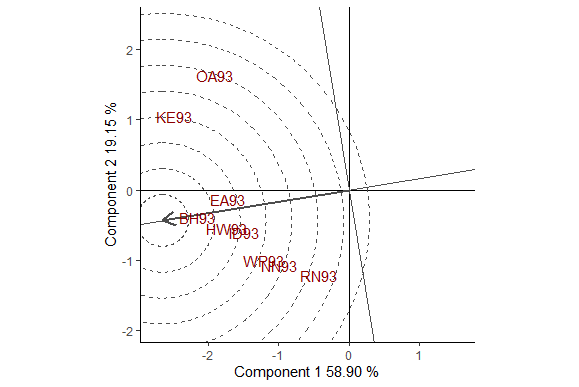
\includegraphics[width=8cm]{./Graficos/RankingEnvironments.png}
	\end{center}
	\caption{Clasificación de ambientes con respecto al ambiente ideal a partir de la función \textcolor{blue}{GGEPlot}()}
\end{figure}
\end{tcolorbox}
\item Clasificación de genotipos con respecto al genotipo ideal.
\begin{tcolorbox}[skin=bicolor,
    colframe=aurometalsaurus,colback=backcolour,colbacklower=white,
    width=1\linewidth,
    height=0.7\linewidth,
    boxsep=-3mm]
\begin{lstlisting}
GGEPlot(GGE1, type = "Ranking Genotypes")
\end{lstlisting}
\tcblower\vskip-\baselineskip
\tcblower
\begin{figure}[H]
	\begin{center}
		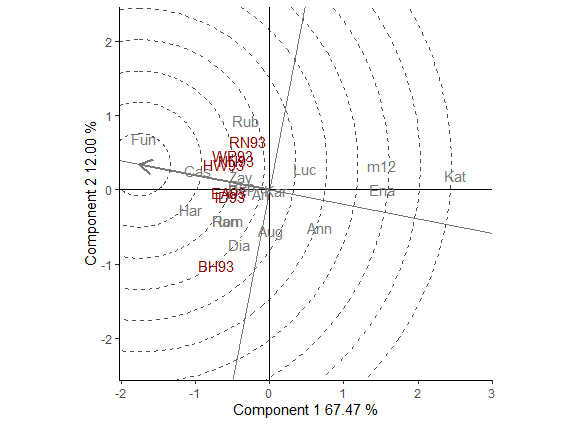
\includegraphics[width=8cm]{./Graficos/RankingGenotypes.png}
	\end{center}
	\caption{Clasificación de genotipos con respecto al genotipo ideal a partir de la función \textcolor{blue}{GGEPlot}()}
\end{figure}
\end{tcolorbox}
\item Evaluación de los cultivares con base en el rendimiento promedio y la estabilidad.
\begin{tcolorbox}[skin=bicolor,
    colframe=aurometalsaurus,colback=backcolour,colbacklower=white,
    width=1\linewidth,
    height=0.7\linewidth,
    boxsep=-3mm]
\begin{lstlisting}
GGEPlot(GGE1, type = "Mean vs. Stability")
\end{lstlisting}
\tcblower\vskip-\baselineskip
\tcblower
\begin{figure}[H]
	\begin{center}
		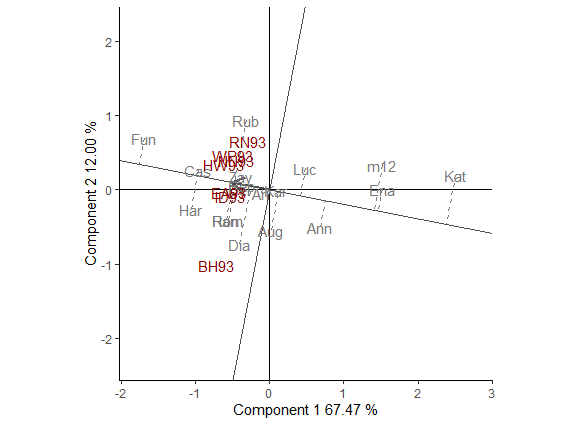
\includegraphics[width=8cm]{./Graficos/MeanvsStability.png}
	\end{center}
	\caption{Evaluación de los cultivares con base en el rendimiento promedio y la estabilidad a partir de la función \textcolor{blue}{GGEPlot}()}
\end{figure}
\end{tcolorbox}
\end{itemize}

\textbf{Classic AMMI model}

Para ejecutar la función \textcolor{blue}{rAMMI}(), como en la función \textcolor{blue}{GGEmodel}(), se debe proporcionar un conjunto de datos con genotipo, entorno, repeticiones (si las hay) y la variable de respuesta. Se debe indicar el nombre de las columnas que contienen cada una de estas variables en el conjunto de datos de entradas. La salida de la función es un biplot.

A continuación se muestra el biplot GE obtenido del modelo AMMI clásico obtenido con el conjunto de datos yan.winterwheat.

\begin{tcolorbox}[skin=bicolor,
    colframe=aurometalsaurus,colback=backcolour,colbacklower=white,
    width=1\linewidth,
    height=0.7\linewidth,
    boxsep=-3mm]
\begin{lstlisting}
rAMMI(dat_yan, genotype = "gen", environment = "env", response = "yield", type = "AMMI")
\end{lstlisting}
\tcblower\vskip-\baselineskip
\tcblower
\begin{figure}[H]
	\begin{center}
		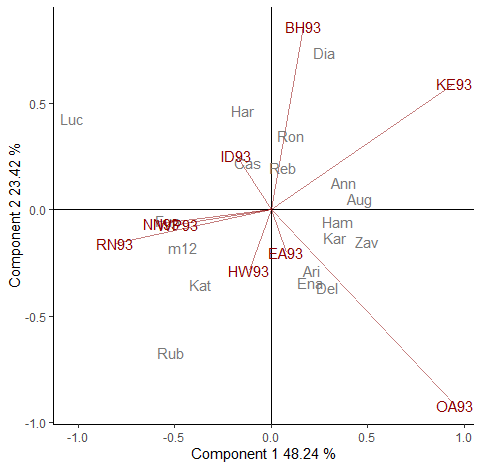
\includegraphics[width=8cm]{./Graficos/AMMI.png}
	\end{center}
	\caption{Biplot GE obtenido del modelo clasico AMMI}
\end{figure}
\end{tcolorbox}

\textbf{Robust AMMI model}

Como se dijo anteriormente, el modelo AMMI clasico, en su forma estándar, no funciona bien en presencia de observaciones atípicas. Dado que los outliers son muy comun en los datos agronómicos, Rodrigues et al. (2015) proponen cinco modelos AMMI robustos, que permiten superar el problema de la contaminación de datos con observaciones atípicas. Los biplots de los cinco modelos AMMI robustos propuestos por Rodrigues et al. (2015), se pueden obtener utilizando la función \textcolor{blue}{rAMMI}() A continuación se muestran los biplots obtenidos con dichos modelos robustos usando el conjunto de datos yan.winterwheat.

\begin{itemize}[wide, nosep, labelindent = 0pt, topsep = 1ex]

\item  modelo "rAMMI"
\begin{tcolorbox}[skin=bicolor,
    colframe=aurometalsaurus,colback=backcolour,colbacklower=white,
    width=1\linewidth,
    height=0.7\linewidth,
    boxsep=-3mm]
\begin{lstlisting}
rAMMI(dat_yan, genotype = "gen", environment = "env", response = "yield", type = "rAMMI")
\end{lstlisting}
\tcblower\vskip-\baselineskip
\tcblower
\begin{figure}[H]
	\begin{center}
		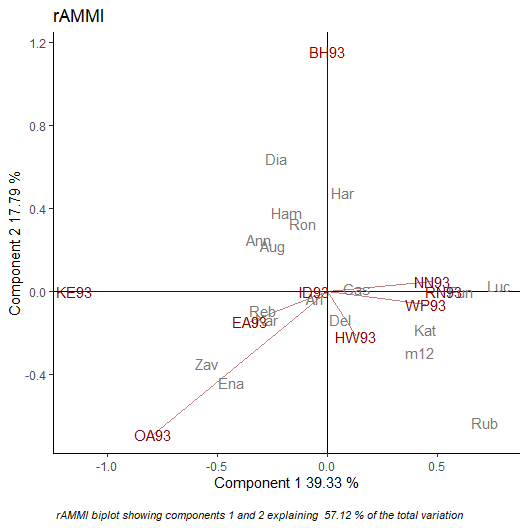
\includegraphics[width=8cm]{./Graficos/rAMMI.png}
	\end{center}
	\caption{Biplot GE obtenido del modelo robusto rAMMI}
\end{figure}
\end{tcolorbox}

\item  modelo "hAMMI"
\begin{tcolorbox}[skin=bicolor,
    colframe=aurometalsaurus,colback=backcolour,colbacklower=white,
    width=1\linewidth,
    height=0.7\linewidth,
    boxsep=-3mm]
\begin{lstlisting}
rAMMI(dat_yan, genotype = "gen", environment = "env", response = "yield", type = "hAMMI")
\end{lstlisting}
\tcblower\vskip-\baselineskip
\tcblower
\begin{figure}[H]
	\begin{center}
		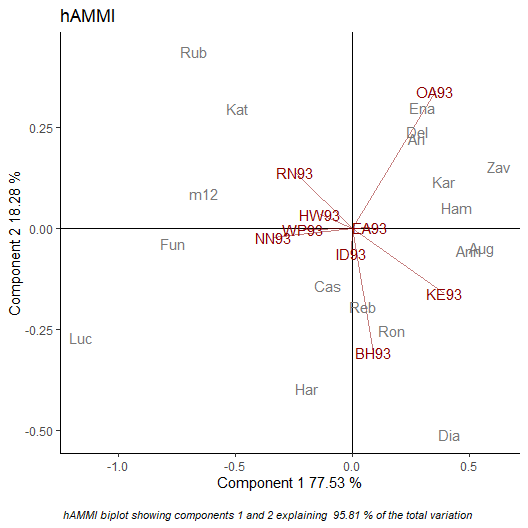
\includegraphics[width=8cm]{./Graficos/hAMMI.png}
	\end{center}
	\caption{Biplot GE obtenido del modelo robusto hAMMI}
\end{figure}
\end{tcolorbox}

\item  modelo "gAMMI"
\begin{tcolorbox}[skin=bicolor,
    colframe=aurometalsaurus,colback=backcolour,colbacklower=white,
    width=1\linewidth,
    height=0.7\linewidth,
    boxsep=-3mm]
\begin{lstlisting}
rAMMI(dat_yan, genotype = "gen", environment = "env", response = "yield", type = "gAMMI")
\end{lstlisting}
\tcblower\vskip-\baselineskip
\tcblower
\begin{figure}[H]
	\begin{center}
		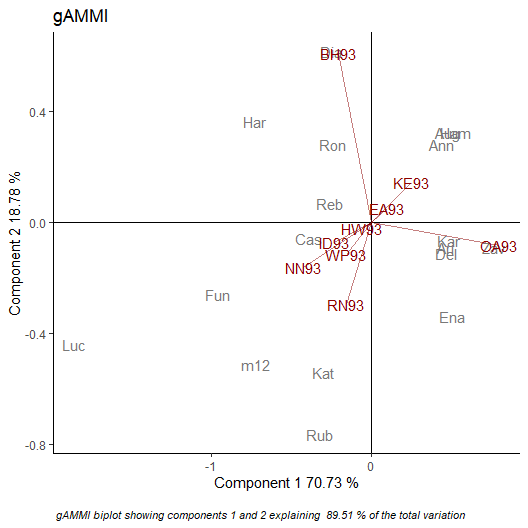
\includegraphics[width=8cm]{./Graficos/gAMMI.png}
	\end{center}
	\caption{Biplot GE obtenido del modelo robusto gAMMI}
\end{figure}
\end{tcolorbox}


\item  modelo "lAMMI"
\begin{tcolorbox}[skin=bicolor,
    colframe=aurometalsaurus,colback=backcolour,colbacklower=white,
    width=1\linewidth,
    height=0.7\linewidth,
    boxsep=-3mm]
\begin{lstlisting}
rAMMI(dat_yan, genotype = "gen", environment = "env", response = "yield", type = "lAMMI")
\end{lstlisting}
\tcblower\vskip-\baselineskip
\tcblower
\begin{figure}[H]
	\begin{center}
		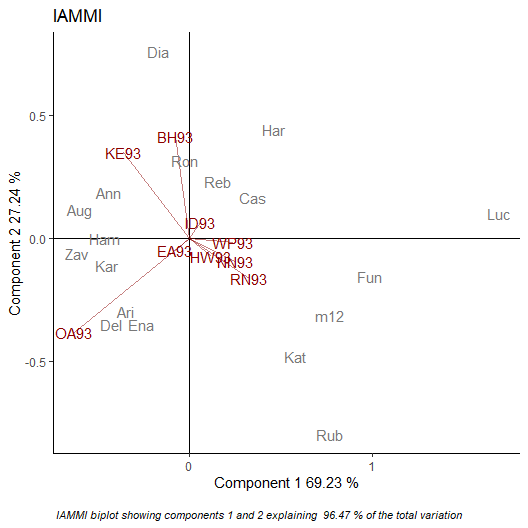
\includegraphics[width=8cm]{./Graficos/lAMMI.png}
	\end{center}
	\caption{Biplot GE obtenido del modelo robusto lAMMI}
\end{figure}
\end{tcolorbox}

\item  modelo "ppAMMI"
\begin{tcolorbox}[skin=bicolor,
    colframe=aurometalsaurus,colback=backcolour,colbacklower=white,
    width=1\linewidth,
    height=0.7\linewidth,
    boxsep=-3mm]
\begin{lstlisting}
rAMMI(dat_yan, genotype = "gen", environment = "env", response = "yield", type = "ppAMMI")
\end{lstlisting}
\tcblower\vskip-\baselineskip
\tcblower

\begin{figure}[H]
	\begin{center}
		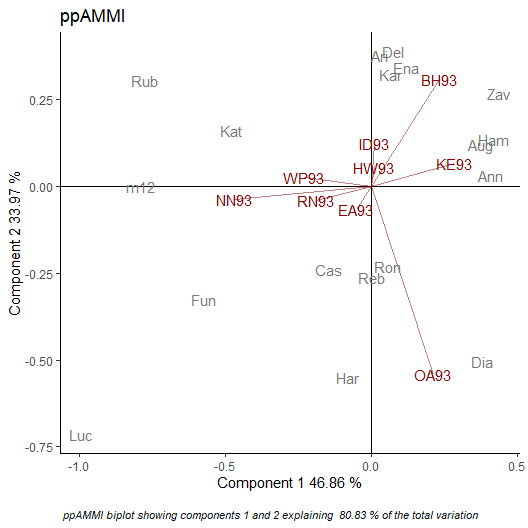
\includegraphics[width=8cm]{./Graficos/ppAMMI.png}
	\end{center}
	\caption{Biplot GE obtenido del modelo robusto ppAMMI}
\end{figure}
\end{tcolorbox}
\end{itemize}

\textbf{Métodos de imputación}

Una limitación importante de los modelos presentados anteriormente es que requieren una que el conjunto de datos este completo. Por lo tanto, en el paquete se incluyen una serie de metodologías propuestas, algunas de las cuales no se encuentran disponible en R, para superar el problema de las observaciones perdidas. 

El conjunto de datos yan.winterwheat se utilizó como ejemplo. Como el conjunto de datos no contaba con observaciones perdidas, algunas fueron eliminadas con el objetivo de mostrar las metodologías de imputación incluidas.
\begin{tcolorbox}[colframe=aurometalsaurus,colback=backcolour,colbacklower=white,
    width=1\linewidth,
    height=0.15\linewidth,
    boxsep=-3mm]
\begin{lstlisting}
# generates missing data
dat_yan[1, 3] <- NA
dat_yan[3, 3] <- NA
dat_yan[2, 3] <- NA
\end{lstlisting}
\end{tcolorbox}

\begin{itemize}[wide, nosep, labelindent = 0pt, topsep = 1ex]
\item GabrielEigein proposed by Arciniegas-Alarcón S., et al. (2010).

\begin{tcolorbox}[skin=bicolor,
    colframe=aurometalsaurus,colback=backcolour,colbacklower=white,
    width=1\linewidth,
    height=0.8\linewidth,
    boxsep=-3mm]
\begin{lstlisting}
imputation(dat_yan, PC.nb = 2, genotype = "gen", environment = "env", response = "yield", type = "EM-AMMI")
\end{lstlisting}
\tcblower\vskip-\baselineskip
\tcblower
\vspace{0.5cm}
\footnotesize\begin{verbatim}
##         BH93  EA93  HW93  ID93  KE93  NN93  OA93  RN93  WP93
## Ann 4.150120 4.150 2.849 3.084 5.940 4.450 4.351 4.039 2.672
## Ari 4.035814 4.771 2.912 3.506 5.699 5.152 4.956 4.386 2.938
## Aug 4.305244 4.578 3.098 3.460 6.070 5.025 4.730 3.900 2.621
## Cas 4.732000 4.745 3.375 3.904 6.224 5.340 4.226 4.893 3.451
## Del 4.390000 4.603 3.511 3.848 5.773 5.421 5.147 4.098 2.832
## Dia 5.178000 4.475 2.990 3.774 6.583 5.045 3.985 4.271 2.776
## Ena 3.375000 4.175 2.741 3.157 5.342 4.267 4.162 4.063 2.032
## Fun 4.852000 4.664 4.425 3.952 5.536 5.832 4.168 5.060 3.574
## Ham 5.038000 4.741 3.508 3.437 5.960 4.859 4.977 4.514 2.859
## Har 5.195000 4.662 3.596 3.759 5.937 5.345 3.895 4.450 3.300
## Kar 4.293000 4.530 2.760 3.422 6.142 5.250 4.856 4.137 3.149
## Kat 3.151000 3.040 2.388 2.350 4.229 4.257 3.384 4.071 2.103
## Luc 4.104000 3.878 2.302 3.718 4.555 5.149 2.596 4.956 2.886
## Reb 4.375000 4.701 3.655 3.592 6.189 5.141 3.933 4.208 2.925
## Ron 4.940000 4.698 2.950 3.898 6.063 5.326 4.302 4.299 3.031
## Rub 3.786000 4.969 3.379 3.353 4.774 5.304 4.322 4.858 3.382
## Zav 4.238000 4.654 3.607 3.914 6.641 4.830 5.014 4.363 3.111
## m12 3.340000 3.854 2.419 2.783 4.629 5.090 3.281 3.918 2.561
\end{verbatim}
\normalsize
\end{tcolorbox}


\item EM-AMMI proposed by Gauch and Zobel (1990).

\begin{tcolorbox}[skin=bicolor,
    colframe=aurometalsaurus,colback=backcolour,colbacklower=white,
    width=1\linewidth,
    height=0.8\linewidth,
    boxsep=-3mm]
\begin{lstlisting}
imputation(dat_yan, PC.nb = 1, genotype = "gen", environment = "env", response = "yield", type = "EM-AMMI")
\end{lstlisting}
\tcblower\vskip-\baselineskip
\tcblower
\vspace{0.5cm}
\footnotesize\begin{verbatim}
##         BH93  EA93  HW93  ID93  KE93  NN93  OA93  RN93  WP93
## Ann 4.136249 4.150 2.849 3.084 5.940 4.450 4.351 4.039 2.672
## Ari 4.474249 4.771 2.912 3.506 5.699 5.152 4.956 4.386 2.938
## Aug 4.386299 4.578 3.098 3.460 6.070 5.025 4.730 3.900 2.621
## Cas 4.732000 4.745 3.375 3.904 6.224 5.340 4.226 4.893 3.451
## Del 4.390000 4.603 3.511 3.848 5.773 5.421 5.147 4.098 2.832
## Dia 5.178000 4.475 2.990 3.774 6.583 5.045 3.985 4.271 2.776
## Ena 3.375000 4.175 2.741 3.157 5.342 4.267 4.162 4.063 2.032
## Fun 4.852000 4.664 4.425 3.952 5.536 5.832 4.168 5.060 3.574
## Ham 5.038000 4.741 3.508 3.437 5.960 4.859 4.977 4.514 2.859
## Har 5.195000 4.662 3.596 3.759 5.937 5.345 3.895 4.450 3.300
## Kar 4.293000 4.530 2.760 3.422 6.142 5.250 4.856 4.137 3.149
## Kat 3.151000 3.040 2.388 2.350 4.229 4.257 3.384 4.071 2.103
## Luc 4.104000 3.878 2.302 3.718 4.555 5.149 2.596 4.956 2.886
## Reb 4.375000 4.701 3.655 3.592 6.189 5.141 3.933 4.208 2.925
## Ron 4.940000 4.698 2.950 3.898 6.063 5.326 4.302 4.299 3.031
## Rub 3.786000 4.969 3.379 3.353 4.774 5.304 4.322 4.858 3.382
## Zav 4.238000 4.654 3.607 3.914 6.641 4.830 5.014 4.363 3.111
## m12 3.340000 3.854 2.419 2.783 4.629 5.090 3.281 3.918 2.561
\end{verbatim}
\normalsize
\end{tcolorbox}


\item EM-SVD proposed by Perry (2009)
\begin{tcolorbox}[skin=bicolor,
    colframe=aurometalsaurus,colback=backcolour,colbacklower=white,
    width=1\linewidth,
    height=0.8\linewidth,
    boxsep=-3mm]
\begin{lstlisting}
imputation(dat_yan, genotype = "gen", environment = "env", response = "yield", type = "EM-SVD")
\end{lstlisting}
\tcblower\vskip-\baselineskip
\tcblower
\vspace{0.5cm}
\footnotesize\begin{verbatim}
##           [,1]  [,2]  [,3]  [,4]  [,5]  [,6]  [,7]  [,8]  [,9]
##  [1,] 4.332467 4.150 2.849 3.084 5.940 4.450 4.351 4.039 2.672
##  [2,] 4.332467 4.771 2.912 3.506 5.699 5.152 4.956 4.386 2.938
##  [3,] 4.332467 4.578 3.098 3.460 6.070 5.025 4.730 3.900 2.621
##  [4,] 4.732000 4.745 3.375 3.904 6.224 5.340 4.226 4.893 3.451
##  [5,] 4.390000 4.603 3.511 3.848 5.773 5.421 5.147 4.098 2.832
##  [6,] 5.178000 4.475 2.990 3.774 6.583 5.045 3.985 4.271 2.776
##  [7,] 3.375000 4.175 2.741 3.157 5.342 4.267 4.162 4.063 2.032
##  [8,] 4.852000 4.664 4.425 3.952 5.536 5.832 4.168 5.060 3.574
##  [9,] 5.038000 4.741 3.508 3.437 5.960 4.859 4.977 4.514 2.859
## [10,] 5.195000 4.662 3.596 3.759 5.937 5.345 3.895 4.450 3.300
## [11,] 4.293000 4.530 2.760 3.422 6.142 5.250 4.856 4.137 3.149
## [12,] 3.151000 3.040 2.388 2.350 4.229 4.257 3.384 4.071 2.103
## [13,] 4.104000 3.878 2.302 3.718 4.555 5.149 2.596 4.956 2.886
## [14,] 4.375000 4.701 3.655 3.592 6.189 5.141 3.933 4.208 2.925
## [15,] 4.940000 4.698 2.950 3.898 6.063 5.326 4.302 4.299 3.031
## [16,] 3.786000 4.969 3.379 3.353 4.774 5.304 4.322 4.858 3.382
## [17,] 4.238000 4.654 3.607 3.914 6.641 4.830 5.014 4.363 3.111
## [18,] 3.340000 3.854 2.419 2.783 4.629 5.090 3.281 3.918 2.561
\end{verbatim}
\normalsize
\end{tcolorbox}


\item WGabriel proposed by Alarcon…..

\begin{tcolorbox}[skin=bicolor,
    colframe=aurometalsaurus,colback=backcolour,colbacklower=white,
    width=1\linewidth,
    height=0.8\linewidth,
    boxsep=-3mm]
\begin{lstlisting}
imputation(dat_yan, genotype = "gen", environment = "env", response = "yield", type = "WGabriel")
\end{lstlisting}
\tcblower\vskip-\baselineskip
\tcblower
\vspace{0.5cm}
\footnotesize\begin{verbatim}
##         BH93  EA93  HW93  ID93  KE93  NN93  OA93  RN93  WP93
## Ann 4.004664 4.150 2.849 3.084 5.940 4.450 4.351 4.039 2.672
## Ari 4.455727 4.771 2.912 3.506 5.699 5.152 4.956 4.386 2.938
## Aug 4.328095 4.578 3.098 3.460 6.070 5.025 4.730 3.900 2.621
## Cas 4.732000 4.745 3.375 3.904 6.224 5.340 4.226 4.893 3.451
## Del 4.390000 4.603 3.511 3.848 5.773 5.421 5.147 4.098 2.832
## Dia 5.178000 4.475 2.990 3.774 6.583 5.045 3.985 4.271 2.776
## Ena 3.375000 4.175 2.741 3.157 5.342 4.267 4.162 4.063 2.032
## Fun 4.852000 4.664 4.425 3.952 5.536 5.832 4.168 5.060 3.574
## Ham 5.038000 4.741 3.508 3.437 5.960 4.859 4.977 4.514 2.859
## Har 5.195000 4.662 3.596 3.759 5.937 5.345 3.895 4.450 3.300
## Kar 4.293000 4.530 2.760 3.422 6.142 5.250 4.856 4.137 3.149
## Kat 3.151000 3.040 2.388 2.350 4.229 4.257 3.384 4.071 2.103
## Luc 4.104000 3.878 2.302 3.718 4.555 5.149 2.596 4.956 2.886
## Reb 4.375000 4.701 3.655 3.592 6.189 5.141 3.933 4.208 2.925
## Ron 4.940000 4.698 2.950 3.898 6.063 5.326 4.302 4.299 3.031
## Rub 3.786000 4.969 3.379 3.353 4.774 5.304 4.322 4.858 3.382
## Zav 4.238000 4.654 3.607 3.914 6.641 4.830 5.014 4.363 3.111
## m12 3.340000 3.854 2.419 2.783 4.629 5.090 3.281 3.918 2.561
\end{verbatim}
\normalsize
\end{tcolorbox}


\item EM-PCA proposed by

\begin{tcolorbox}[skin=bicolor,
    colframe=aurometalsaurus,colback=backcolour,colbacklower=white,
    width=1\linewidth,
    height=0.8\linewidth,
    boxsep=-3mm]
\begin{lstlisting}
imputation(dat_yan, genotype = "gen", environment = "env", response = "yield", type = "EM-PCA")
\end{lstlisting}
\tcblower\vskip-\baselineskip
\tcblower
\vspace{0.5cm}
\footnotesize\begin{verbatim}
##         BH93  EA93  HW93  ID93  KE93  NN93  OA93  RN93  WP93
## Ann 3.980317 4.150 2.849 3.084 5.940 4.450 4.351 4.039 2.672
## Ari 4.463093 4.771 2.912 3.506 5.699 5.152 4.956 4.386 2.938
## Aug 4.327731 4.578 3.098 3.460 6.070 5.025 4.730 3.900 2.621
## Cas 4.732000 4.745 3.375 3.904 6.224 5.340 4.226 4.893 3.451
## Del 4.390000 4.603 3.511 3.848 5.773 5.421 5.147 4.098 2.832
## Dia 5.178000 4.475 2.990 3.774 6.583 5.045 3.985 4.271 2.776
## Ena 3.375000 4.175 2.741 3.157 5.342 4.267 4.162 4.063 2.032
## Fun 4.852000 4.664 4.425 3.952 5.536 5.832 4.168 5.060 3.574
## Ham 5.038000 4.741 3.508 3.437 5.960 4.859 4.977 4.514 2.859
## Har 5.195000 4.662 3.596 3.759 5.937 5.345 3.895 4.450 3.300
## Kar 4.293000 4.530 2.760 3.422 6.142 5.250 4.856 4.137 3.149
## Kat 3.151000 3.040 2.388 2.350 4.229 4.257 3.384 4.071 2.103
## Luc 4.104000 3.878 2.302 3.718 4.555 5.149 2.596 4.956 2.886
## Reb 4.375000 4.701 3.655 3.592 6.189 5.141 3.933 4.208 2.925
## Ron 4.940000 4.698 2.950 3.898 6.063 5.326 4.302 4.299 3.031
## Rub 3.786000 4.969 3.379 3.353 4.774 5.304 4.322 4.858 3.382
## Zav 4.238000 4.654 3.607 3.914 6.641 4.830 5.014 4.363 3.111
## m12 3.340000 3.854 2.419 2.783 4.629 5.090 3.281 3.918 2.561
\end{verbatim}
\normalsize
\end{tcolorbox}
\end{itemize}

\section{Geneticae Shiny Web App}

La aplicación Geneticae permite a los usuarios realizar alguno de los análisis incluidos en el paquete geneticae. La misma se organiza en las siguientes pestañas:
\begin{itemize}[wide, nosep, labelindent = 0pt, topsep = 1ex]
\item Los datos
\item Análisis descriptivo
\item ANOVA
\item Biplot GGE
\item Biplot GE
\item Ayuda
\end{itemize}

En muchos casos, algunos atributos estilísticos de salida pueden personalizarse para que el usuario obtenga la salida a su gusto. A su vez, los gráficos obtenidos pueden ser descargados.


\subsection{Los datos}
Al iniciar la aplicación Geneticae, se muestra una pantalla en la cual se carga el conjunto de datos a analizar. La aplicación admite datos en formato .csv, delimitados por coma o punto y coma; y permite el siguiente formato de datos: 
\begin{itemize}[wide, nosep, labelindent = 0pt, topsep = 1ex]
\item Cada fila contiene una observación, en la cual deben estar presentes los siguientes datos: nombre del cultivar, ambiente, repetición si está disponible y valor fenotipico medido. Pueden estar presentes otras variables que no serán utilizadas por la aplicación.
\item La primera fila de encabezado contiene los nombres de cada variable. Los encabezados pueden dar cualquier nombre que elija, y deben indicarse al cargar el archivo de datos.
\item El número de repeticiones puede diferir con los genotipos y los ambientes.
\end{itemize}

Se utilizan dos conjuntos de datos, incluidos en el paquete geneticae, para ilustrar la aplicación. Estos conjuntos de datos, uno de los cuales tiene repeticiones (plrv dataset) y el otro no (yan.winterwheat dataset), los cuales se pueden ver y descargar en la pestaña \emph{The data} $\rightarrow$ \emph{Example datasets} (Figura \ref{fig:fig41},\ref{fig:fig42}). 

\begin{figure}[H]
	\begin{center}
		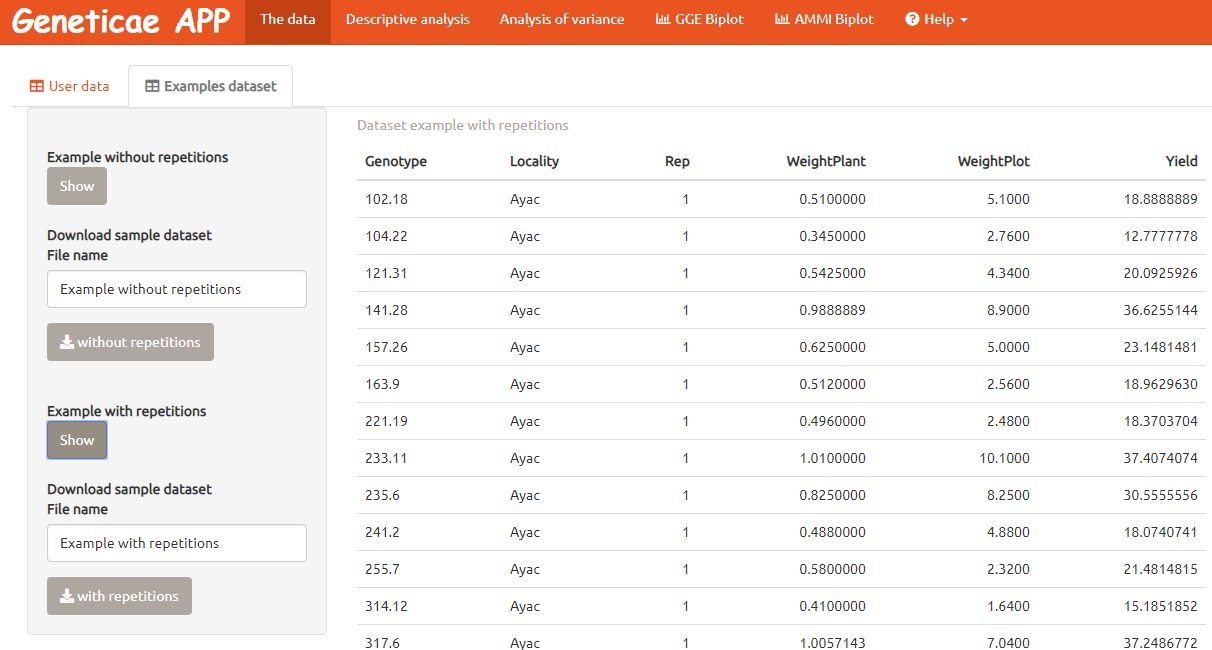
\includegraphics[width=16cm]{./Graficos/Exampledatasets_withoutrep.png}
	\end{center}
	\caption{yan.winterwheat dataset disponible en Shiny Web App}
	\label{fig:fig41}
\end{figure}


\begin{figure}[H]
	\begin{center}
		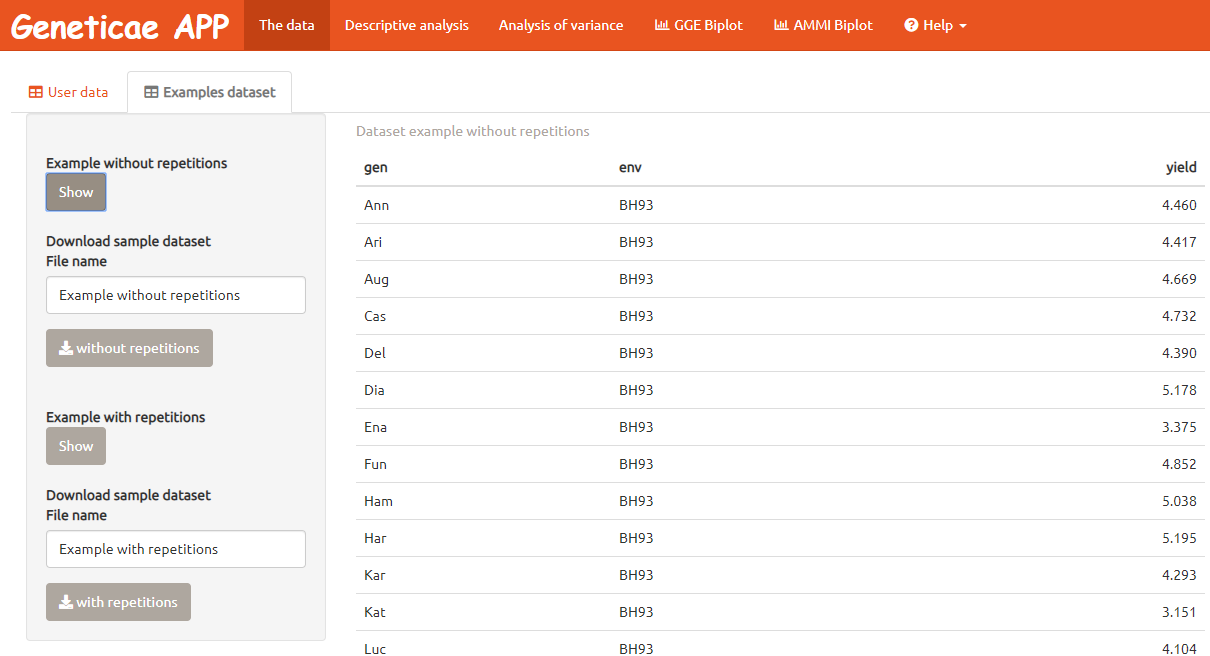
\includegraphics[width=16cm]{./Graficos/Exampledatasets_withrep.png}
	\end{center}
	\caption{plrv dataset disponible en Shiny Web App}
	\label{fig:fig42}
\end{figure}

\subsection{Análisis descriptivo}

El menú \emph{Descriptive analysis} le permite describir un conjunto de datos utilizando diagrama de caja (o \emph{boxplot}), gráfico y matriz de correlación y gráfico de interacción.

\subsubsection{\emph{Boxplot}}
El \emph{boxplot} proporciona una medida central, la mediana y una idea de la dispersión a través del rango y el rango intercuartil. La posición de la mediana dentro de la caja y la similitud en la longitud de los bigotes nos dan una idea de la simetría de la distribución. 

Un boxplot intetactivo que compara el caracter cuantitativo de interés a través de genotipos, así como a través de los ambientes se pueden obtener (Figura \ref{fig:fig43},\ref{fig:fig44}). A partir de los mismos se pueden obtener medidas resumen en forma interactiva usando el \emph{Toggle Spike Lines} como se muestra en la figura \ref{fig:fig43}. Estos gráficos se pueden descagar en formato interactivo (.HTML) a partir del boton \emph{Download} (Figura \ref{fig:fig43} y \ref{fig:fig44}), así como también en formato .png como se muestra en la Figura \ref{fig:fig44}.

\begin{figure}[H]
	\begin{center}
		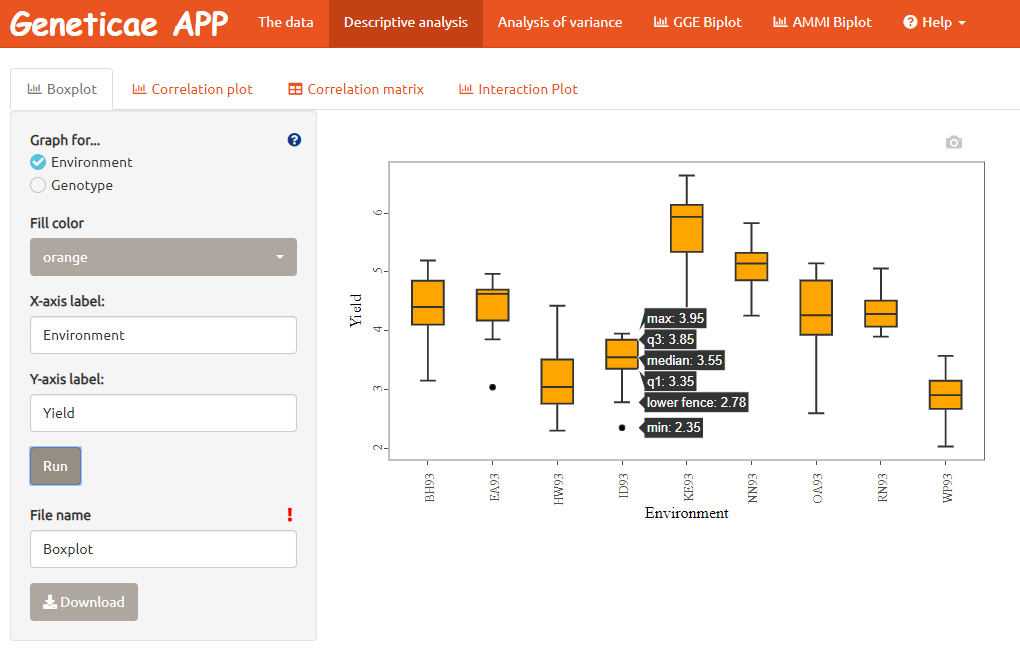
\includegraphics[width=16cm]{./Graficos/Boxplot_environment.png}
	\end{center}
	\caption{Boxplot de ambientes a través de los genotipos para el conjunto de datos Plrv}
	\label{fig:fig43}
\end{figure}


\begin{figure}[H]
	\begin{center}
		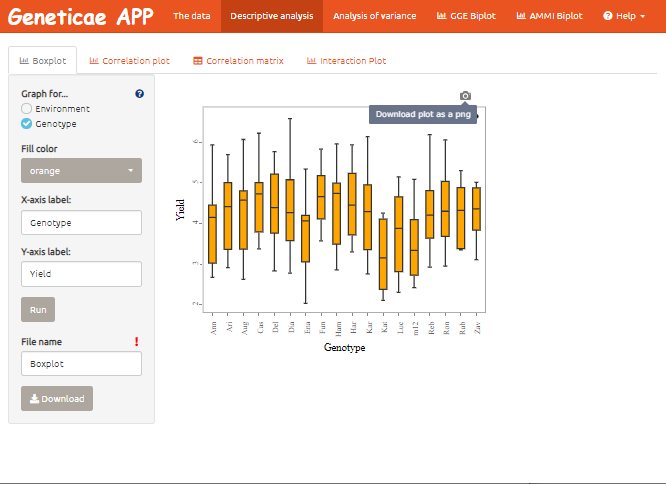
\includegraphics[width=16cm]{./Graficos/Boxplot_genotypes.png}
	\end{center}
	\caption{Boxplot de genotipos a través de los ambientes para el conjunto de datos Plrv}
	\label{fig:fig44}
\end{figure}

\subsubsection{Gráfico de correlación}
El correlograma o gráfico de correlación muestra la correlación tanto entre los genotipos como entre los ambientes (Figura \ref{fig:fig45} y \ref{fig:fig46}). Se pueden mostrar las correlaciones de Pearson y Spearman. Las correlaciones positivas se muestran en azul y las negativas en rojo. La intensidad del color y el tamaño del círculo son proporcionales a los coeficientes de correlación. 


\begin{figure}[H]
	\begin{center}
		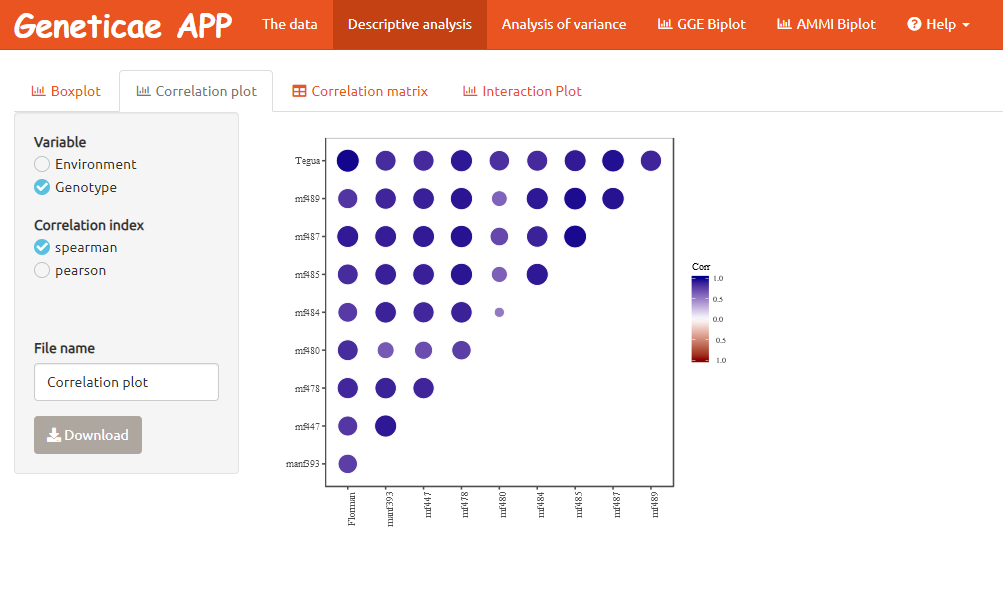
\includegraphics[width=16cm]{./Graficos/corr_gen.png}
	\end{center}
	\caption{Boxplot de genotipos a través de los ambientes para el conjunto de datos Plrv}
	\label{fig:fig45}
\end{figure}


\begin{figure}[H]
	\begin{center}
		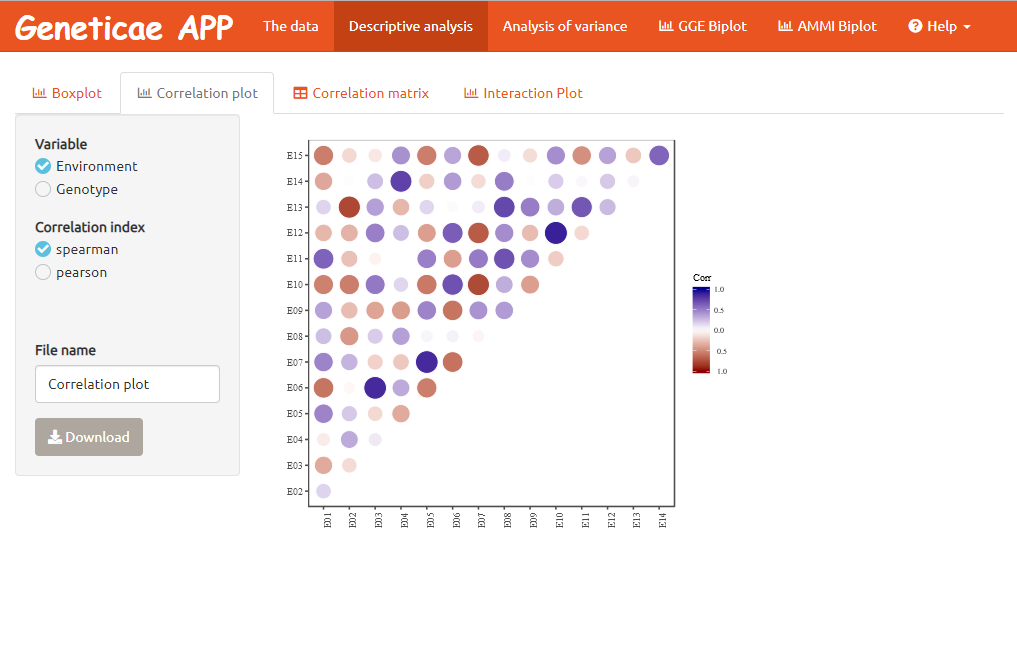
\includegraphics[width=17cm]{./Graficos/corr_withrep.png}
	\end{center}
	\caption{Boxplot de ambientes a través de los genotipos para el conjunto de datos Plrv}
	\label{fig:fig46}
\end{figure}

\subsubsection{Matriz de correlación}
Una matriz de correlación se utiliza como una forma de resumir datos. Muestra los coeficientes de correlación de pares de variables. Las correlaciones de Spearman o Pearson se pueden calcular tanto para ambientes como para genotipos (Figura \ref{fig:fig47}).


\begin{figure}[H]
	\begin{center}
		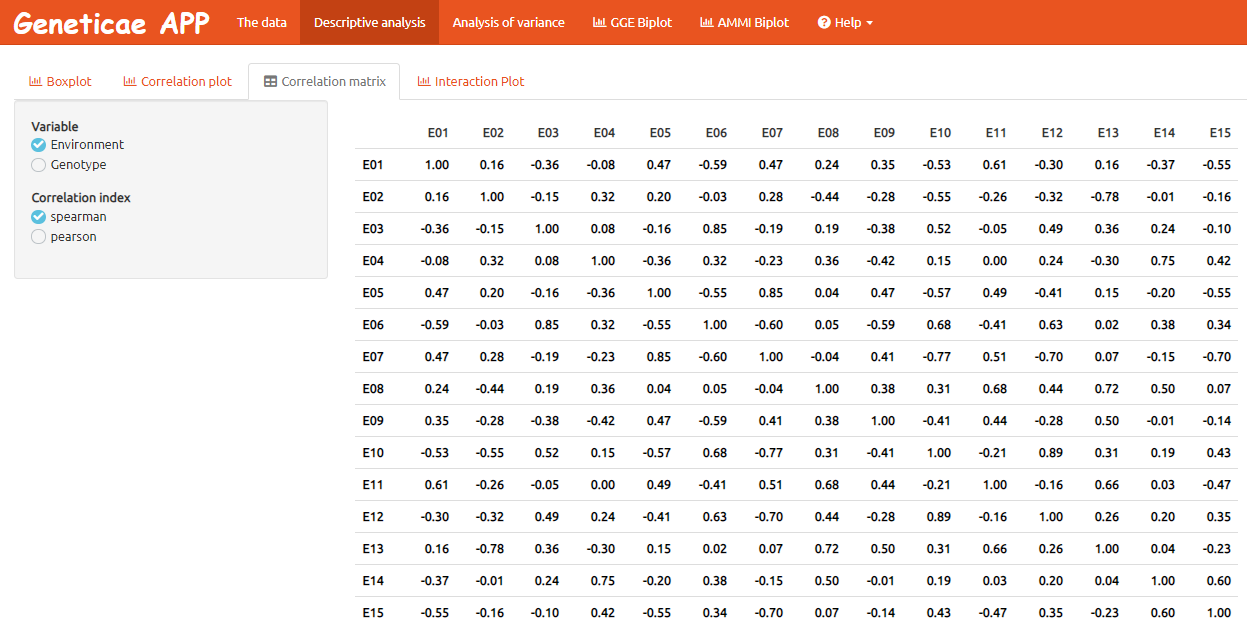
\includegraphics[width=17cm]{./Graficos/corr_matrix.png}
	\end{center}
	\caption{Boxplot de genotipos a través de los ambientes para el conjunto de datos Plrv}
	\label{fig:fig47}
\end{figure}



\subsubsection{Gráfico de interacción}
Un diagrama de interacción es una representación visual de la interacción entre los efectos de dos factores, o entre un factor y una variable numérica. 

Se puede obtener el gráfico interactivo que muestra el cambio en el efecto genotípico a través de los entornos y también el que muestra el cambio en el efecto ambiental a través de los genotipos (Figura \ref{fig:fig49},\ref{fig:fig410}). Es posible descargarlo en formato interactivo (.HTML) a partir del boton \emph{Download} (Figura \ref{fig:fig49}), así como también en formato .png como se muestra en la Figura \ref{fig:fig410}.


\begin{figure}[H]
	\begin{center}
		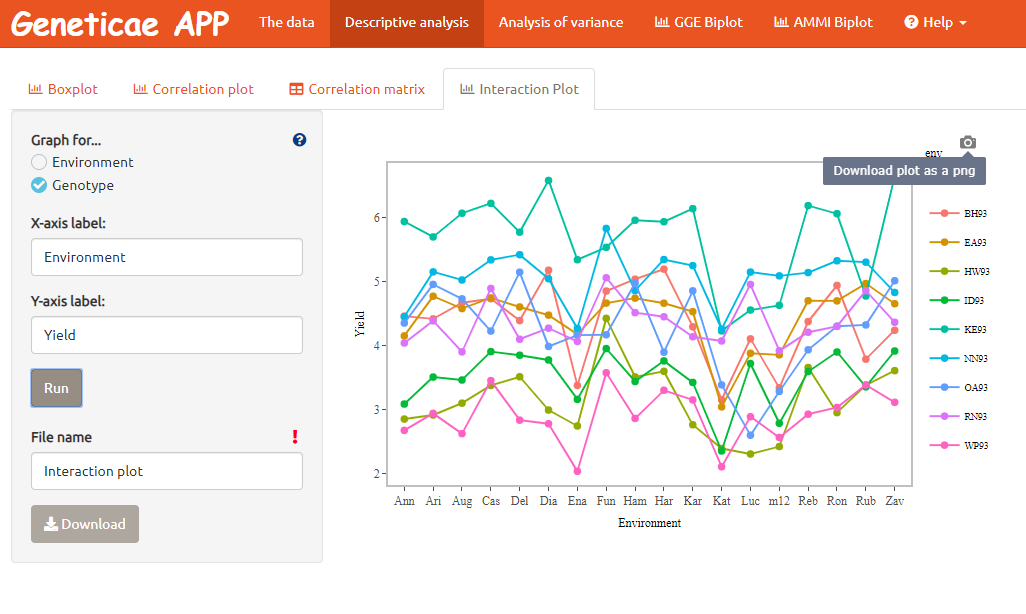
\includegraphics[width=17cm]{./Graficos/int_plot.png}
	\end{center}
	\caption{Boxplot de genotipos a través de los ambientes para el conjunto de datos Plrv}
	\label{fig:fig49}
\end{figure}



\subsection{Análisis de la variancia}

Cuando se pretende llevar a cabo el análisis de la variancia si el conjunto de datos tiene repeticiones entonces saldrá un mensaje en el cual se aclara que la interacción puede ser testada debido a la presencia de repeticiones "The interaction effect can be tested since there are repetitions in the data set", si no hay repeticiones disponibles entonces el mensaje será que la interacción no puede testarse.

\begin{figure}[H]
	\begin{center}
		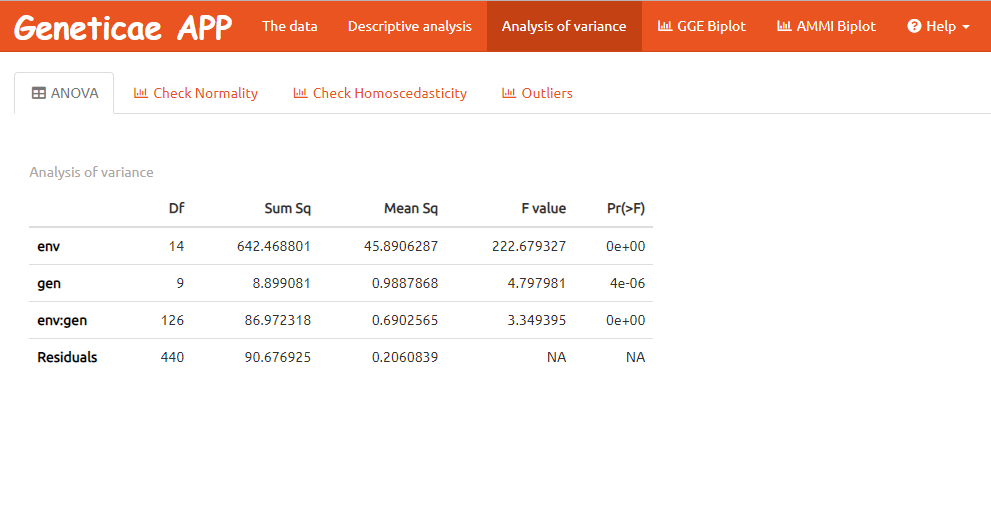
\includegraphics[width=17cm]{./Graficos/ANOVA.png}
	\end{center}
	\caption{Boxplot de genotipos a través de los ambientes para el conjunto de datos Plrv}
	\label{fig:fig49}
\end{figure}


El ANOVA depende del cumplimiento de los supuestos de que los errores tengan distribución normal con media cero y variancia constante. Por ello, tres pestañas: \emph{Check normality}, \emph{Check homocedasticity} y \emph{Outliers} se encuentran disponibles para la verificación de los supuestos mencionados.

Para verificar el supuesto de normalidad, se puede realizar un histograma, un gráfico de probabilidad normal y la prueba de shapiro-wilks sobre los residuos del ANOVA.

\begin{figure}[H]
	\begin{center}
		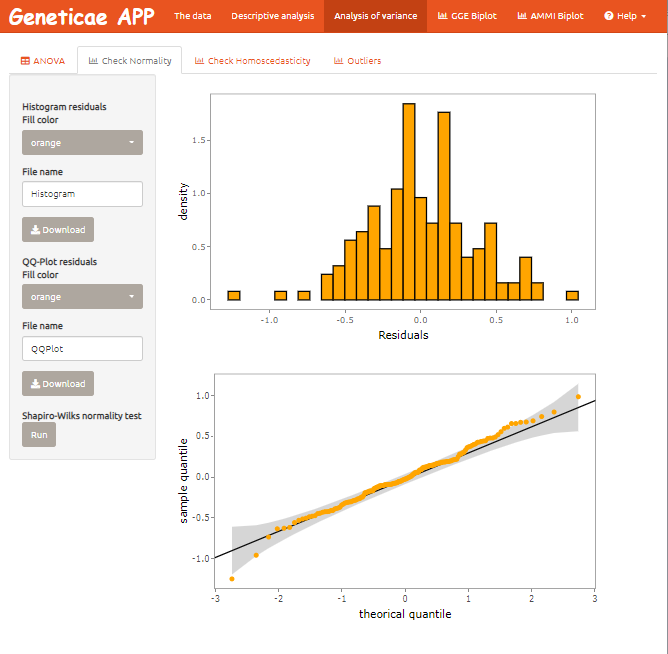
\includegraphics[width=17cm]{./Graficos/Normalidad.png}
	\end{center}
	\caption{Boxplot de genotipos a través de los ambientes para el conjunto de datos Plrv}
	\label{fig:fig49}
\end{figure}

El grafico de residuos vs. valores predichos y las pruebas de levene permiten verificar el supuesto de variancia constante u homocedasticidad.

\begin{figure}[H]
	\begin{center}
		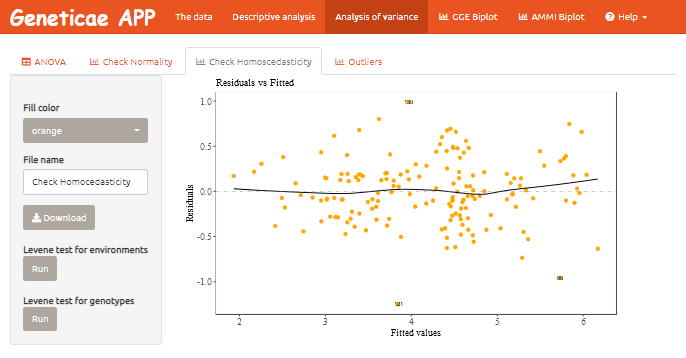
\includegraphics[width=17cm]{./Graficos/Homocedasticidad.png}
	\end{center}
	\caption{Boxplot de genotipos a través de los ambientes para el conjunto de datos Plrv}
	\label{fig:fig49}
\end{figure}

Por último, la presencia de observaciones atipicas u outliers provoca que el ANOVA no de buenos resultados, un grafico para detectar outliers es posible realizarlo.

\begin{figure}[H]
	\begin{center}
		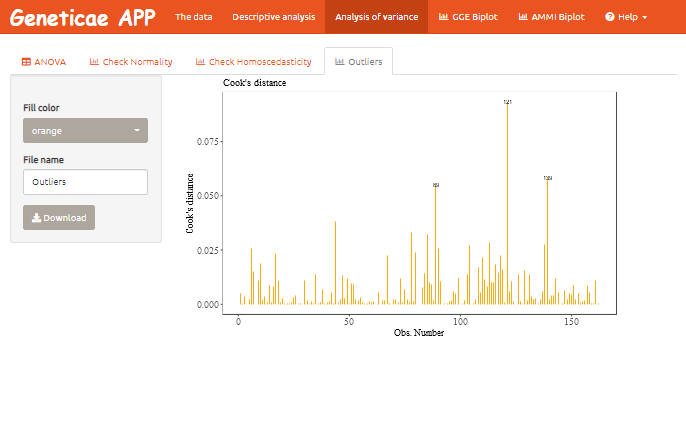
\includegraphics[width=17cm]{./Graficos/Outliers.png}
	\end{center}
	\caption{Boxplot de genotipos a través de los ambientes para el conjunto de datos Plrv}
	\label{fig:fig49}
\end{figure}

\subsection{Biplot GGE}
El biplot GGE aborda visualmente muchos problemas relacionados con la evaluación de los genotipo y ambientes de prueba. En el caso de repeticiones disponibles en el conjunto de datos, se obtiene el valor fenotípico promedio para cada combinación de genotipo y ambiente. Los valores faltantes no están permitidos.


\subsection{Biplot GE}

